\documentclass{scrartcl}

\usepackage{siunitx}
\usepackage{graphicx}
\usepackage{caption}
\usepackage{glossaries}
\usepackage[english]{babel}
\usepackage{booktabs}
\usepackage[linktoc=all,hidelinks]{hyperref}
\usepackage{fontspec}
% \usepackage{authblk}
\usepackage{unicode-math}

% \makeatletter
% \renewcommand\AB@affilsepx{,~ \protect\Affilfont}
% \makeatother

\setkomafont{author}{\sffamily}

\newcommand{\nump}[2]{\num[round-mode=places,round-precision=#2]{#1}}
\DeclareGraphicsExtensions{.pdf,.eps}
\bibliographystyle{unsrt}

\title{Report}
\subtitle{A study of machine learning algorithms for reconstruction of missing energy in particle physics experiments.}
% \subject{Statistical Machine Learning}

\author{
  Max Isacson, \url{max.isacson@physics.uu.se}
  \and
  Mikael M\aa rtensson, \url{mikael.martensson@physics.uu.se}
  \and
  Camila Rangel Smith, \url{camila.rangel@physics.uu.se}
  \and
  Henrik Öhman, \url{ohman@cern.ch}
}
% \author[1]{Max Isacsson}
% \author[2]{Mikael M\aa rtensson}
% \author[3]{Camila Rangel Smith}
% \author[4]{Henrik \"{O}hman}
% \affil[1]{\small\url{max.isacsson@physics.uu.se}}
% \affil[2]{\url{mikael.martensson@physics.uu.se}}
% \affil[3]{\url{camila.rangel@physics.uu.se}}
% \affil[4]{\url{ohman@cern.ch}}

\newacronym{NN}{NN}{Neural Network}

\newcommand{\etmiss}{$E_\mathrm{T}^\text{miss}$}
\newcommand{\exmiss}{$E_x^\text{miss}$}
\newcommand{\eymiss}{$E_y^\text{miss}$}

\begin{document}
\maketitle

% \begin{figure}
%     \centering
%     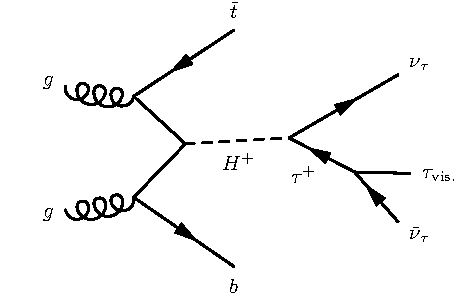
\includegraphics[width=.7\textwidth]{fig/heavyHplustaunu4fs.pdf}
%     \caption{Feynman diagram of the production and decay of a charged Higgs boson. Not shown is the hadronic top decay $\bar t \to \bar b W^-(q \bar q')$.}\label{fig:hplus}
% \end{figure}

\section{Introduction}

\section{The Dataset}
\subsection{Structure}
The dataset consists of simulated $pp$ collision events, in which a charged Higgs is produced and decays as $H^+\to\tau\nu$. Each event is described by one set of observable variables and one set of unobservable variables.

Observable variables:
\begin{itemize}
    \item \exmiss, \eymiss --- The $x$- and $y$-components of the missing energy.
    \item $P_{\tau_\mathrm{vis.}}$ --- The 4-momentum of the visible (hadronic) part of the $\tau$ decay.
    \item $P_{b_0}$, $P_{b_1}$, $P_{q_0}$, $P_{q_1}$ --- The 4-momenta of the two $b$-jets and two light jets.
\end{itemize}

Unobservable variables:
\begin{itemize}
    \item $P_{\nu_\tau}$ --- The 4-momentum of the neutrino from the charged Higgs decay.
    \item $P_{\bar\nu_\tau}$ --- The 4-momentum of the neutrino from the $\tau$ decay.
\end{itemize}

\subsection{Production}
MG5\_aMC@NLO \cite{Alwall:2014hca} is used for the matrix element computation of $gg / q \bar q \to H^+$ and the event simulation. The events are then passed to PYTHIA8 \cite{Sjöstrand2015159} for the showering and hadronization, and for the $H^+\to \tau\nu$ decay. Finally, the detector response is simulated using DELPHES \cite{Favereau2014} with an ATLAS-like geometry.

\subsection{Estimated and true quantities}
The true quantities for both the observable and the unobservable variables are available as output from the event simulation. The estimated values for the observable variables are reconstructed from the output from the detector response simulation.

\section{Solution method}

\subsection{Predictor selection}

\subsection{Neural Network}

\subsubsection{Data scaling}
% There are two scaling schemes commonly used for Neural Networks In the first scheme, the data is scaled to have a mean of 0 and a standard deviation of 1. In the second scheme the minimum of the dataset is set to -1 and the maximum to 1. Scaling the data in this way improves the training performance by avoiding the flat tails of the activation functions.

In this study, the dataset was scaled such that the training set mean was set to 0 and the standard deviation 1 to for each input variable $x_i$ and the training target $t_{\text{tr}}$:

% The input $x_i$ (both the validation set and the training set) for the individual predictor variables $i$ and the training set target $t_{\text{tr}}$ is normalized by setting the mean $\mu$ to 0 and standard deviation $\sigma$ to 1 using the training set data:

\begin{align}
  \label{eq:nnxnorm}
  x_i' &= \frac{x_i - \mu(x_{i,\text{tr}})}{\sigma(x_{i,\text{tr}})},\\
  \label{eq:nntnorm}
  t_{\text{tr}}' &= \frac{t_{\text{tr}} - \mu(t_{\text{tr}})}{\sigma(t_{\text{tr}})}.
\end{align}

\noindent This improves the training performance by avoiding the flat tails of the activation functions. The reverse of equation \ref{eq:nntnorm} is then applied to the \gls{NN} prediction of the validation $t_\text{val}'$ to get the physical output $t_\text{val}$:

\begin{equation}
  t_\text{val} = t_\text{val}'\sigma(t_\text{tr}) + \mu(t_\text{tr})
\end{equation}

\subsubsection{Implementation}
The python package Keras \cite{keras} was used to implement neural networks. The number of input nodes is restricted to the 25 selected predictor variables and the output to the target dimension of 1. Also, since the network is used for regression, the output activation function must be linear. A large number of configurations of the hidden layers were tested by varying the number of layers, the number of perceptrons in each layer, and the activation functions (sigmoid, tanh, softmax, and relu). 


\section{Results}

\bibliography{refs}

\end{document}
